Po przetwarzaniu wstępnym obrazu, kolejnym krokiem algorytmu wykrywania logo \bk była konwersja przestrzeni barw z~RGB do przestrzeni~HSV.

\subsection{Przestrzeń RGB}
Najbardziej znanym modelem przestrzeni barw jest model opisywany współrzędnymi RGB. Nazwa współrzędnych pochodzi od pierwszych liter nazw barw podstawowych: \textbf{R} - czerwona, \textbf{G} - zielona oraz \textbf{B} - niebieska. Model ten bazuje na właściwościach ludzkiego oka. Wrażenie widzenia dowolnej barwy można uzyskać poprzez zmieszanie trzech wiązek światła \cite{jankowski1990elementy}.

Model RGB jest domyślnie wykorzystywany w~informatyce do przechowywania plików graficznych. Wykorzystywana w~rozwiązaniu biblioteka OpenCV, również bazuje na tym modelu, odwracając kolejność kolorów. Zamiast jako pierwszą przechowywać informację o kolorze czerwonym, pierwsza przechowywana informacja mówi o~kolorze niebieskim, tak jak zostało to przedstawione na rysunku~\ref{fig:bgr}. Tak odwróconą przestrzeń nazywa się przestrzenią BGR~\cite{opencv}.

\begin{figure}[h]
    \centering
    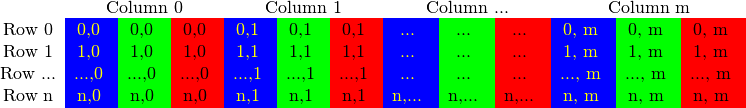
\includegraphics[width=\columnwidth]{./figures/opencv-matrix-bgr.png}
    \caption{Sposób reprezentacji obrazu w~przestrzeni BGR, wykorzystywanej w~OpenCV~\cite{opencv}}
    \label{fig:bgr}
\end{figure}

\subsection{Przestrzeń HSV}
Model HSV czerpie swoją nazwę od pierwszych liter angielskich nazw składowych: \textbf{H} - hue (barwa), \textbf{S} - saturation (nasycenie), \textbf{V} - value (wartość). Model ten znacznie różni się od poprzednio omawianego modelu. W~RGB, wszystkie trzy zmienne niosą jednocześnie informację na temat chrominancji (kolorze) i~luminancji (jasności) punktu. W~modelu HSV, tylko jedna składowa \textbf{V} niesie informację o~jasności piksela a~pozostałe dwie zmienne \textbf{H}~i~\textbf{S}~przechowują informację o~chrominancji piksela. Taki sposób reprezentacji znacznie ułatwia wykrywanie na zdjęciu obiektów o~danej barwie lecz o~różnym oświetleniu. Typowo, przestrzeń HSV przedstawia się za pomocą stożka, zaprezentowanego na rysunku~\ref{fig:hsv}.

\begin{figure}[h]
    \centering
    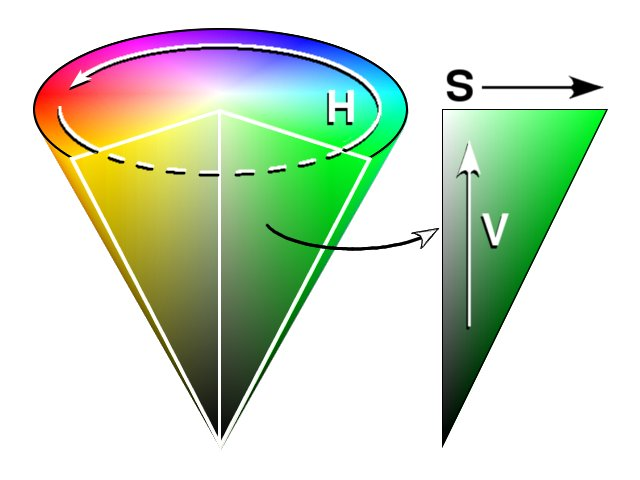
\includegraphics[width=0.6\columnwidth]{./figures/HSV_cone.jpg}
    \caption{Stożek przestrzeni barw HSV~\cite{WikipediaPL:hsvCone}}
    \label{fig:hsv}
\end{figure}   

Podobnym modelem do HSV jest model HSL (\textit{Hue, Saturation, Lightness}). Oba modele jednakowo definiują zmienną barwową H, natomiast różnią się w~definicji pozostałych zmiennych. Największe różnice zachodzą w~definicji jasności/wartości koloru. W~modelu HSV, wartość $0\%$ reprezentuje kolor czarny, natomiast wartość $100\%$ kolor w pełni nasycony. W~modelu HSL, w~pełni nasycone kolory mają wartość jasności $50\%$, natomiast kolory czarny i~biały mają odpowiednio $0\%$ oraz $100\%$. Mimo iż model HSL bardziej intuicyjnie przedstawia jasność koloru, uznałem że bardziej odpowiedni do automatycznego przetwarzania będzie model HSV.

\subsection{Implementacja konwersji}
Konwersja piksela w~modelu RGB $(R, G, B)$ do modelu HSV $(H,S,V)$ jest operacją punktową i~nie wymaga informacji na temat wartości innych pikseli. W~programie, konwersję przeprowadza obiekt klasy \texttt{POBR::BGR2HSVConverter}.  

Zaimplementowany algorytm konwersji bazuje na podstawowym algorytmie z~OpenCV~\cite{opencv-conversions}. Pierwszym jego krokiem jest obliczenie jasności $V$, zgodnie ze wzorem \ref{eqn:value}.
\smallskip
\begin{equation}
    \label{eqn:value}
    V = \max{(R, G, B)}
\end{equation}

Kolejnym krokiem algorytmu, jest obliczenie nasycenia koloru $S$, korzystając ze wzoru~\ref{eqn:saturation}.

\begin{equation}
    \label{eqn:saturation}
    S = \left\{ 
        \begin{array}{ll}
            0, & V = 0 \\
            \min{(R, G, B)}, & V \ne 0
        \end{array} 
        \right.
\end{equation}

Ostatnim krokiem algorytmu jest obliczenie barwy $H$~zgodnie z~wzorem~\ref{eqn:hue}.

\begin{equation}
    \label{eqn:hue}
    H = \left\{ 
        \begin{array}{ll}
            \frac{(G - B) * 60\si{\degree}}{V - \min{(R, G, B)}} + 60\si{\degree}, & V = R \\
            \frac{(B - R) * 60\si{\degree}}{V - \min{(R, G, B)}} + 120\si{\degree}, & V = G \\
            \frac{(R - G) * 60\si{\degree}}{V - \min{(R, G, B)}} + 240\si{\degree}, & V = B
        \end{array} 
        \right.
\end{equation}
\smallskip

Wartości zmiennych $V$~i~$S$ mieszczą się w~przedziale $[0; 255]$ natomiast wartości zmiennej $H$ są ograniczone przez przedział $[0; 360]$. Obrazy przechowywane są tablicy o~ośmiobitowym rozmiarze podstawowym \texttt{uchar}. Zmienna $H$ nie mieści się w~komórce o~tym rozmiarze, dlatego też zdecydowałem się na przechowywanie w~tablicy wartości $\frac{H}{2}$. Podział ten jest solidnym kompromisem pomiędzy dokładnością reprezentacji a~rozmiarem obrazu w~pamięci komputera. Jest on również domyślnie wykorzystywany w~reprezentacji obrazów w~modelu~HSV w~bibliotece OpenCV~\cite{opencv}.